
\documentclass[12pt, letterpaper, twoside]{article}
\usepackage[utf8]{inputenc}
\usepackage[russian]{babel}
\usepackage{graphicx}
\graphicspath{ {images/} }


 
\title{Теоретический материал по физике}
\author{Макаров Иван ИКМО-03-20 \thanks{Спасибо Советову Петру Николаевичу в помощи разработки в  системе LaTeX}}
\date{Октябрь 2021}

\begin{document}

\maketitle

\begin{center}    \qquad 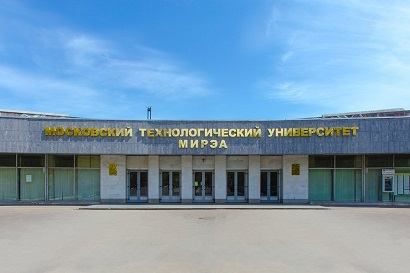
\includegraphics{zvt11.png}
\end{center}


\begin{center} Статья написана в \LaTeX{} document!
\end{center}



\newpage
\begin{center}
    \textbf{Закон всемирного тяготения}\\

\end{center}



\textbf{Формулировка:} Между любыми двумя материальными точками массами m и M действует гравитационная сила взаимного притяжения, направленная вдоль прямой, соединяющей эти точки. Величина этой силы прямо пропорциональна произведению масс этих точек и обратно пропорциональна квадрату расстояния r между ними.\\
\begin{center}
    $F=G\frac{mM}{r^2}$\\
\end{center}

\textit{Коэффициент пропорциональности G  называется гравитационной постоянной и равен} $6.67 \cdot 10^{-11}$ $\frac{M^3}{KG \cdot C^{-2}}$.\\

\begin{center}    \qquad 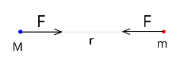
\includegraphics{zvt1.png}
 
\end{center}


Закон всемирного тяготения имеет обобщение и для случая сферической симметрии, итак:
\textit{Между любой парой сферически симметричных тел, центры тяжести которых разнесены на расстояние много большее, чем сумма их радиусов, по линии соединяющей их центры тяжести, действует гравитационная сила взаимного притяжения, зависящая прямо пропорционально от произведения масс этих тел, и обратно пропорционально от квадрата расстояния между их центрами тяжести.\\}

\begin{center}
$F=G\frac{mM}{r^2}$\\
\end{center}


\begin{center}
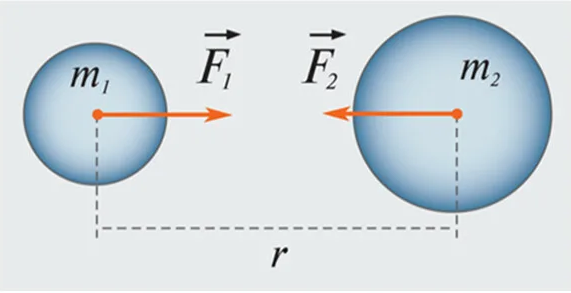
\includegraphics{zvt2.png} \\

\end{center}



\begin{center}
    \textbf{Сила тяжести} \\
\end{center}

Рассмотрим однородную планету массой M и радиусом R. На её поверхности лежит тело массой m. На него действует гравитационная сила со стороны планеты. Эту силу будем называть силой тяжести. Сила тяжести есть частный случай силы всемирного тяготения на поверхности планеты.
Будем считать планету идеальным, однородным шаром, тогда сможем сконцентрировать всю ее массу в геометрический центр и рассматривать планету как материальную точку с соответствующей массой. Тогда тело массой m на поверхности планеты, удален от ее центра на расстояние R км, воспользуемся случаем для пары материальных точек 
\begin{center}
   $F=G\frac{mM}{r^2}$\\
\end{center}

	Заметим, что для для любого небесного тела величина
$G\frac{M}{R^2}$ постоянна на всей поверхности планеты, обозначим ее как g и проверив размерности, обнаружим, что g имеет размерность ускорения. Перепишем закон всемирного тяготения с учетом переобозначения//
\begin{center}
   $F=mg$\\

\end{center}

Получаем уже хорошо известную нам формулу для силы тяжести на поверхности земли.

Итак сформулируем определение для силы тяжести:\\
\textit{Сила тяжести - есть, ни что иное как, сила гравитационного взаимодействия планеты на все тела у ее поверхности.}
\begin{center}
   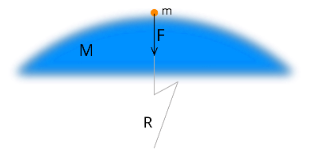
\includegraphics{zvt3.png} \\

\end{center}


Определение можно расширить, подняв тело на расстояние H от поверхности, ускорение свободного падения
\begin{center}
   $g_{eff} = G\frac{M}{(R+H)^2}$
\end{center}


Здесь, можно ввести такое понятие как эффективная сила тяжести,т.е сила с которой планета действует на тело массой m поднятое на расстояние H от границы 
\begin{center}
  $F=mg_{eff}$
\end{center}
\begin{center}
   \qquad 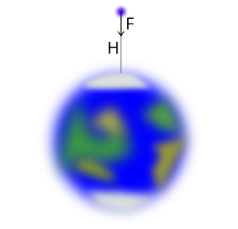
\includegraphics{zvt4.png}\\
\end{center}



Таким образом, мы логично приходим к следующему умозаключению. \textit{Сила тяжести индивидуальна для каждой планеты, и кроме того зависит от расстояния до поверхности планеты от центра тяжести рассматриваемого тела.}
\begin{center}
  \textbf{Для экзаменах в государственных учереждениях } 
\end{center}

В экзаменах принято считать ускорение свободного падения на поверхности равным 10  если в условии задачи не оговорено обратного.




\end{document} % конец документа